% !Mode:: "TeX:UTF-8"
\chapter{视频编码原理与关键技术}
\label{cha:c2}
本章由简要的视频编码技术发展史开始,引出视频编码中最为核心的 5 项技术:预测编码、变换量化 (Transform and Quantization, TransQuant)、环路后处理、熵编码以及率-失真优化 (Rate-Distortion Optimization, RDO),为后文分析视频编码的可优化方向以及分析所提出算法的可行性打下基础。在早期视频编码标准中并未包含上述所有核心技术,但随着各类应用对视频编码效率的需求日渐严苛,该 5 项核心技术被证明对编码效率提高起着核心作用,成为了缺一不可的存在。目前仍在征集提案的 H.266 标准的发展趋势亦是在该框架下再进行部分精细的优化。

在正文之前,首先申明以下用词:1) 统一使用视频“编码”而非视频“压缩”。在视频编解码领域,“编码”与“压缩”表达相同的含义,都指经过预测、变换量化、熵编码等操作达到减小数据冗余、压缩视频数据量的目的。编码是手段,压缩是目的,按照习惯统一使用视频编码这一表述,类似地,使用编码标准、编码方案、编码效率等表述;2) 为了直接体现出编码标准的发展历程,不使用高级视频编码 (Advanced Video Coding, AVC)、高性能视频编码 (High Efficiency Video Coding, HEVC) 和多功能视频编码 (Versatile Video Coding, VVC) 的表述,统一使用 H.264、H.265 和 H.266,两类表述在含义上并无差异;3) 由联合专家组维护的各标准参考模型随着版本迭代可能存在不同的命名,例如 H.266 的参考模型在早期曾称为 JEM(Joint Exploration Model),本文中统一使用以下命名:用于 H.264 的 JM(Joint Test Model) 模型、用于 H.265 的 HM(HEVC Test Model) 模型以及用于 H.266 的 VTM(VVC Test Model) 模型。

\section{视频编码技术发展历史}
从上世纪 80 年代开始
\begin{figure}[htb]
    \centering
    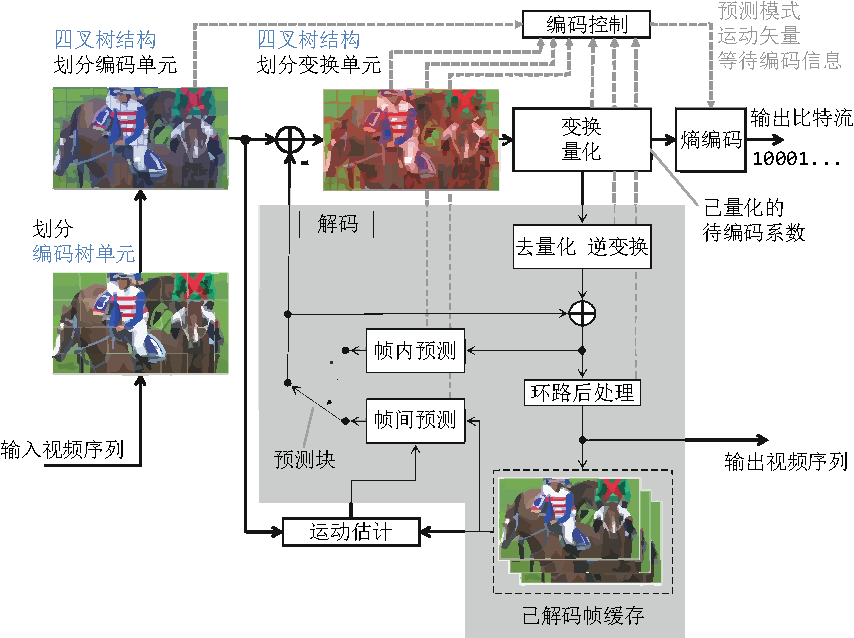
\includegraphics{BlockDiagram.pdf}
    \caption{H.26X 标准视频编码框架}
    \label{fig:BlockDiagram}
\end{figure}

\section{预测编码技术}
预测编码是 H.26X 系列编码标准中的重要组成部分之一。视频信号表现出很强的空间相关性和时间相关性,即在空间上相邻像素点之间的亮度或色差值相近,在时间上同一区域相邻两帧之间的像素点亮度或色差值相近。使用帧内和帧间预测技术可以准确地对待编码数据进行预测,进而编码预测值与原始像素值的残差,极大地减少视频信号的时空冗余。预测编码的基本流程如图 \ref{fig:PredicitonOverview} 所示。对于待预测像素 $x(n)$,首先利用已重建的像素结合特定的预测模式得到预测值 $p(n)$,然后计算预测残差 $e(n)$,最后对 $e(n)$ 进行变换、量化、熵编码,同时使用去量化、逆变换后的重建值 $e^{'}(n)$ 与预测值 $p(n)$ 重建出后续待预测像素的参考值 $x^{'}(n)$。
\begin{figure}[htb]
    \centering
    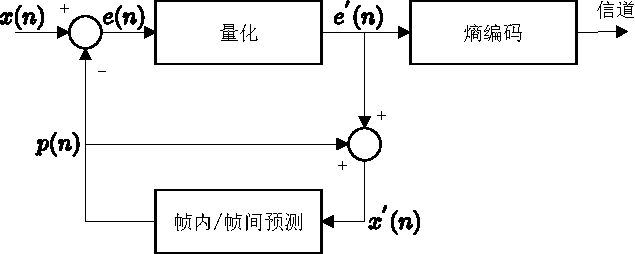
\includegraphics{PredicitonOverview.pdf}
    \caption{H.26X 预测编码的基本流程}
    \label{fig:PredicitonOverview}
\end{figure}

根据参考像素种类的不同,可将预测编码分为以下两类,在后文将进一步介绍:
\begin{enumerate}
    \item 帧内预测,即利用待预测点空间上临近的已重建像素点进行预测的方法;
    \item 帧间预测,即利用待预测点时间上临近的几帧(可以是之前也可以是之后)在相同位置附近的已重建像素点进行预测的方法。
\end{enumerate}

\subsection{帧内预测}
帧内预测指利用视频、图像的空间相关性,使用已编码重建的像素点预测当前像素,预测完成后的像素经过重建又作为后续待预测像素的参考点。设待预测点为 $f(x,y)$,$(x,y)$ 为待预测点坐标,该点的预测值由已重建的参考点 $\widetilde{f}(k,l)$ 进行预测给出:
\begin{equation}
    \widehat{f}(x,y) = \sum_{(k,l)\in Z}a_{k,l}\widetilde{f}(k,l)
\end{equation}
其中 $a_{k,l}$ 表示特定的预测方式,多表现为投影与插值的组合,$Z$ 为参考点所在的区域,包含坐标 $(k,l)$。后续变换量化、熵编码的对象均为预测值与真实值的误差,即预测残差 $e(x,y)$:
\begin{equation}
    e(x,y) = f(x,y) - \widehat{f}(x,y) 
\end{equation}

H.26X 系列标准中制定了多种帧内预测模式,包括平滑预测(DC 模式、Planar 模式)和方向预测两大类。随着编码标准的发展,预测模式的数量不断增多,H.264 仅使用 9 种模式\upcite{H264Overview},H.265 增加到 35 种\upcite{H265Overview},H.266 达到了 67 种\upcite{H266Overview},显然模式越多越有可能得到精确的预测值,最后体现为更高的编码效率。标准中,任意一种预测模式都是以相邻块的边界上的重建像素为参考点进行的,该方案使得每个预测单元均能自适应地选择最佳的预测模式。如图 \ref{fig:ModeFit} 所示,左侧衣物上存在明显的方向性条纹,适合使用方向预测模式,而右侧的衣物呈现出平坦的特性,适合使用 DC 或 Planar 模式。关于帧内预测的更详细的分析将在 \ref{cha:IntraPredDetail} 节进行。
\begin{figure}[htb]
    \centering
    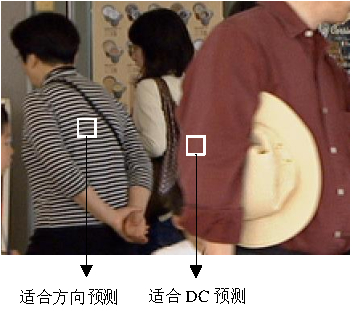
\includegraphics{ModeFit.pdf}
    \caption{选择不同的帧内预测模式}
    \label{fig:ModeFit}
\end{figure}

\subsection{帧间预测}
帧间预测指利用视频的时间相关性,使用临近帧(可以是之前也可以是之后)相同位置附近的像素点预测当前像素。以像素点为单位进行帧间预测显然是不可行的,因此与帧内预测类似帧间预测也使用以块为单位的运动补偿技术,如图 \ref{fig:InterPredOverview} 所示。其预测策略是针对每个待预测块,从已编码的其他帧中寻找与其匹配的块作为参考块,计算参考块到待预测块的位移信息。该过程即为运动估计,其中得到的位移信息称为运动矢量,预测块与参考块的差值称为运动预测残差。
\begin{figure}[htb]
    \centering
    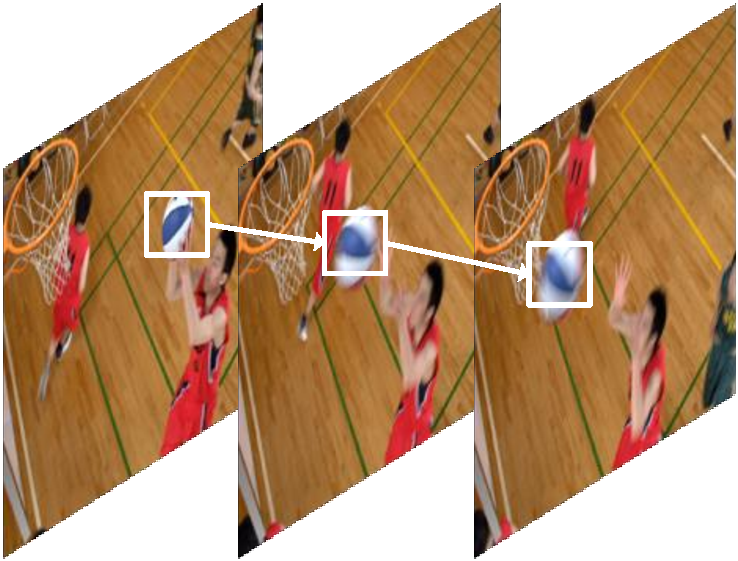
\includegraphics[scale=0.7]{InterPredOverview.pdf}
    \caption{H.26X 帧间预测}
    \label{fig:InterPredOverview}
\end{figure}

帧间预测中的核心技术是运动搜索算法,运动搜索是 H.26X 编码中最耗时但也是影响编码效率最大的一个过程。H.26X 标准中并未指定搜索方法而只在软件模型中给出了参考算法,例如 HM 模型中给出了全搜索算法和 TZSearch 算法\upcite{ImprovementsTZSearch}。全搜索算法指对于每一个待预测块,遍历搜索窗口中所有可能的运动矢量取其中运动预测残差最小的一个;TZSearch 算法属于快速算法的一种,其按照固定的菱形搜索模板或正方形搜索模板以 2 的整数次幂递增步长进行运动搜索,大幅减少搜索量的同时保持了较好的搜索性能(不容易陷入局部最优)。

\section{变换与量化技术}
H.26X 编码标准中,通过帧内和帧间预测获得了相对原始像素值能量大幅降低的预测残差,且预测编码并未引入失真。后续的变换与量化进一步地对残差进行处理,使能量集中得到稀疏的待编码数据,同时也是编码过程中真正引入失真的步骤。
\subsection{变换编码}
\label{cha:TransformOverview}
变换编码技术指将预测残差(某些特殊情况下是原始像素值)从空间域通过离散余弦变换 (Discrete Cosine Transform, DCT) 或离散正弦变换 (Discrete Sine Transform, DST) 转换到频域,以变换系数来表示数据。本节以 DCT 为例简单介绍 H.26X 标准中变换编码的应用场景及效果。

DCT 是一种在频域对数字信号进行分析的工具,在数学上共有 8 种形式\upcite{FastFourierTransform},图像、音视频领域中常用的是 II 类 DCT:
\begin{equation}
    \begin{gathered}
        X(k) = \sqrt{\frac{2}{N}}\varepsilon_{k}\sum_{n=0}^{N-1}x(n)\cos\left[\frac{k(2n+1)\pi}{2N}\right], \quad k=0,1...,N-1 \\
        \varepsilon_{k}= \left\{
        \begin{aligned}
            \frac{1}{\sqrt{2}}, \quad &k=0 \\
            1, \quad &o.w
        \end{aligned} \right.
    \end{gathered}
    \label{equ:1ddct}
\end{equation}
当 $k=0$ 时式中不再有余弦项,即 $X(0)\propto$ 信号 $x(n)$ 的均值,此时称 $X(0)$ 为信号 $x(n)$ 的直流 (Direct Current, DC) 分量;反之,当 $k>0$ 时,$k$ 越大式中的余弦信号频率越高,此时 $X(k)$ 反映了信号 $x(n)$ 在不同频率分量上的分布多寡,称为信号 $x(n)$ 的交流 (Alternate Current, AC) 分量。

以 H.265 标准测试序列“BasketballPass”中第一帧的前 8 个数据 $x(n)$ 为例计算其对应的变换域系数 $X(k)$:
\[
    x(n): 127,129,130,128,125,122,123,124
\]
当 $k=0$ 时:
\[
    X(0)=\frac{1}{2\sqrt{2}}(127+129+130+128+125+122+123+124)\cos(0)\approx 356
\]
同理根据式 \ref{equ:1ddct} 计算所有的 $X(k)$ 得到:
\[
    X(k): 356,6,-1,-4,0,0,0,0
\]
从上述示例中可以看出,当原始信号 $x(n)$ 的数值分布比较均匀即各数值之间相关性强时,其变换域的系数表示 $X(k)$ 将呈现出数值集中分布在 DC 和低频部分的稀疏状态。显然,自然图像中的像素幅值或其预测残差都很容易表现出强相关性,因此将待编码数据转换到变换域十分有利于后续的熵编码。另外,上述示例是 II 类 DCT 的一维形式,实际上图像、视频编码中使用的是其二维形式:
\begin{equation}
    \begin{gathered}
        X(k,l)=C(k)C(l)\sum_{m=0}^{N-1}\sum_{n=0}^{N-1}x(m,n)\cos\left[\frac{(2m+1)k\pi}{2N}\right]\cos\left[\frac{(2n+1)l\pi}{2N}\right], \\
        % k,l=0,1...,N-1
        C(k)=C(l)= 
        \begin{cases}
            \sqrt{\frac{1}{N}}, \quad k,l=0 \\
            \sqrt{\frac{2}{N}}, \quad 1 \leqslant k,l \leqslant N-1
        \end{cases}
    \end{gathered}
    \label{equ:2ddct}
\end{equation}

变换编码技术在 H.26X 中存在较多研究和优化内容不再赘述,但以下几点值得一提:
\begin{enumerate}
    \item DCT 去相关性的性能随着变换大小的增大而增强,但增强的比率迅速减缓,因此考虑到计算复杂度和编码性能的折衷,较常采用的是 4x4 与 8x8 DCT,很少用到 16x16 及更大的变换;
    \item 同样出于计算复杂度的考虑,从 H.264 开始标准中的变换一般拆分为两部分进行,即与浮点运算无关的整数变换部分及分离出的比例缩放系数\upcite{IntergerDCTs},后者将与量化合并为一次计算,提高了计算效率;
    \item 根据统计结果,对 4x4 大小的亮度块预测残差使用 DST 能提高约 0.8\% 的编码效率而计算复杂度不变\upcite{DCTDSTchoose},因此从 H.265 开始将 DST 纳入考虑;
    \item 哈达玛变换与 DCT 处理后的变换残差绝对值之和 (Sum of Absolute Transformed Difference, SATD) 相近,但哈达玛变换计算复杂度极低,因此 H.265 将哈达玛变换与 SATD 作为快速预测模式选取的工具。
\end{enumerate}

\subsection{量化}
从 H.264 将变换拆分为整数变换和比例缩放两部分以后,H.26X 标准中产生失真的原因集中到了量化上(图 \ref{fig:TransQuantCombine})。H.26X 标准中仅规定了量化过程的解码方法,将编码端量化方式的选择策略交给编码器自行设计和优化,H.265 中可选的量化方法有传统标量量化、自适应量化 (Adaptive Quantization) 和率-失真优化量化 (Rate-Distortion Optimization Quantization, RDOQ),本节以标量量化为例介绍量化的过程和作用。 
\begin{figure}[htb]
    \centering
    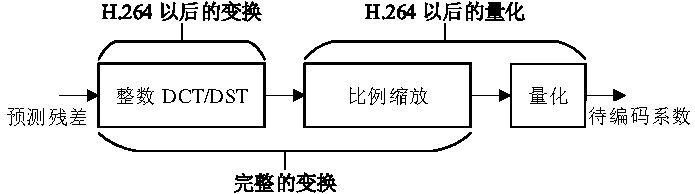
\includegraphics{TransQuantCombine.pdf}
    \caption{H.26X 中变换量化过程的拆分与合并}
    \label{fig:TransQuantCombine}
\end{figure}

由于经过变换后的数据动态范围很大,需要通过量化将数据的取值范围压缩才能得到理想的编码效率。经过压缩必定会产生数据精度损失,因此量化是音视频编码中产生失真的根本原因,也是控制编码结果码率的最直接因素。标量量化的过程如下式:
\begin{equation}
    l_i=\left\lfloor \frac{c_i}{Q_{step}}+f \right\rfloor
\end{equation}
其中 $c_i$ 表示 \ref{cha:TransformOverview} 节所述的变换域系数,$Q_{step}$ 为量化步长,$l_i$ 为量化器的输出,$f$ 用于控制舍入。H.265 中可选 52 个量化步长,量化步长小代表数据精度损失小即失真小但同时编码效率低。需要注意量化并非简单地对输入的变换域系数平等地做缩放。基于人类视觉系统 (Human Visual System, HVS) 研究中发现的人眼对亮度、低频分量敏感,对色差、高频分量较不敏感的生物特性,各类图像视频编码方案中均存在量化矩阵的概念。即对不同频率分量的变换域系数做相应的缩放,例如对低频分量做更轻微的量化以保证良好的视觉效果。值得一提的是相对于学术界关注峰值信噪比 (Peak Signal-to-Noise Ratio, PSNR)、结构相似度 (Structural Similarity Index, SSIM) 等客观图像质量评价指标,工业界更关心的是平均主观得分 (Mean Opinion Score, MOS),即实验者根据自身的观看体验给出的图像视频质量分数,工业界中甚至有关于“让人感觉舒服,错以为图像质量好的失真”的研究,此为另外的研究方向不再展开。总之量化是控制视频质量的关键步骤,量化系数的选择策略尤为重要。

\section{环路后处理技术}
H.26X 标准中的预测、变换和量化等编码工具均是基于块设计的,相邻块之间由于预测模式突变、量化值突变和不属于同一个变换单元等多方面原因,产生了不可避免的数值不连续性。针对
\subsection{去方块滤波}
\begin{figure}[htb]
    \centering
    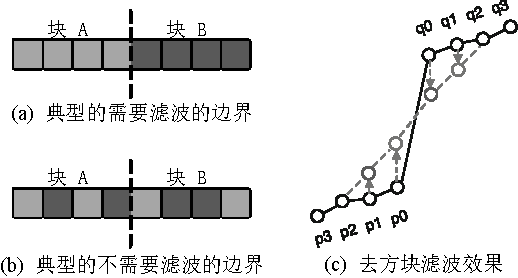
\includegraphics{TypicalDB.pdf}
    \caption{去方块滤波应用场景及效果}
    \label{fig:TypicalDB}
\end{figure}

\subsection{样点自适应补偿}

\section{熵编码技术}
\subsection{变长编码在视频编码中的应用}
\subsection{算术编码在视频编码中的应用}
\subsection{模式依赖的编码顺序}

\section{率-失真优化技术}
不论是视频编码标准还是各类网络传输协议标准,标准中制定的往往只是各类语法和语义(部分包含同步规则和检错纠错规则),只要是符合标准语法语义的码流都能称为符合某视频编码标准。例如在使用 H.265 进行编码时,若将最小预测单元限定为 32x32(HM 默认配置是 4x4),编码效率与失真度可以预见甚至不如简单的 M-JPEG(Motion Joint Photographic Experts Group)。因此,如何在标准的编码框架下得到最优的编码效率与失真度的平衡是编码算法研究的核心内容之一,寻找折衷点的过程被称为率-失真优化。
% 有各种级别的率-失真优化,片层级,CTU 级,PU 级
% 不同的软件有不同的方案,介绍 HM
% 标准只规定了码流语义 编码可以自由发挥 就算我全用64x64质量超低也能叫HEVC 所以需要优秀的压缩率-失真的折衷策略
% 也是业界在竭力优化的核心内容

\section{软、硬件视频编码开源项目}
互联网开源精神是当今学术界与工业界发展的重要推手,而视频编解码这一涉及到成像系统、生物信息、数学、统计学、计算机以及集成电路的庞大学科,如果没有一个系统的开源项目让各学科的研究人员参与进来,而是由单一的某一组织闭门造车是无法得到长足发展的。本小节总结了目前常用的软、硬件视频编码开源项目,本课题就是基于其中部分项目开展的。
\subsection{软件视频编码开源项目}
\begin{itemize}
    \item JM\upcite{AVCsoftwareJM}

    JM 是制定 H.264 标准的联合开发组 (Joint Video Team, JVT) 负责维护的 H.264 编解码参考软件。JM 是学术界常用的编码器,其实现了 H.264 的所有特性,内部没有使用多线程或进行汇编层级的优化,因此其编解码速度较慢无法实现实时编码,多用于研究和测试标准性能。

    \item x264

    x264 是由 VideoLAN 维护的 H.264 编码器。x264 是工业界最常用的 H.264 编码器,其内部集成了丰富的快速、并行算法,使得编解码效率得到了极大提升,被应用在各类开源音视频处理框架中。目前最完善的多媒体处理软件 FFmpeg 在 H.264 部分就内嵌了 x264 用于编码。

    \item HM\upcite{HEVCsoftwareHM16}

    HM 是制定 H.265 标准的视频编码联合工作组 (Joint Collaborative Team on Video Coding, JCT-VC) 负责维护的 H.265 编解码参考软件。HM 是学术界在研究 H.265 和下一代视频编码标准时常用的编码器,其实现了 H.265 的所有特性(包括部分未写入标准的会议提案),内部没有使用多线程或进行汇编层级的优化,因此其编解码速度较慢无法实现实时编码,多用于研究和测试标准性能。

    \item VTM\upcite{VVCsoftwareVTM}

    VTM 是制定 H.266 标准的联合视频探索小组 (Joint Video Exploration Team, JVET) 负责维护的 H.266 编解码参考软件,随着 H.266 编码提案的征集仍在快速迭代中,在 H.266 标准探索的初期曾称为 JEM。VTM 是联合小组在制定下一代视频编码标准 H.266 时使用的编码器,用于测试编码提案的性能。

    \item VVenC\upcite{VVCsoftwareVVenC}
    
    VVenC(Fraunhofer Versatile Video Encoder) 是在考虑到 VTM 过于庞大冗杂的编码工具后,根据多种复杂度优化提案在编码性能和编码时间之间取折衷的 H.266 编码器。维护者来自 VTM 开发的主要参与方、H.266 标准制定的重要参与者 Fraunhofer HHI。
\end{itemize}

\subsection{硬件视频编码开源项目}
\begin{itemize}
    \item OpenASIC Encoder RTL IP

    OpenASIC H.264/H.265 Encoder RTL IP 是由复旦大学微电子学院视频图像处理科研团队发布的 H.264/H.265 开源 RTL IP,由开源芯片社区 OpenASIC 共同维护。其中 H.264 Encoder RTL IP 实现了 H.264 标准编码流程,最大支持 1920x1088@30fps 实时编码,已被部分公司、研究所研究使用;H.265 Encoder RTL IP 发布了 2 个版本,实现了帧内/帧间预测、熵编码、环路后处理以及基础的码率控制,满足 0.13$\mu$m 工艺 400MHz 无时序违例综合,最大支持 4K@30fps 实时编码。
\end{itemize}

\section{本章小结}